	\chapter{One effect deletion -oe}
	
	This reduction is aimed to remove redundant invariants from operations. Firstly, action having effect of type $<u_i,u_j>$ ($u_i$ is not -1) can be used at most once in case that there is no action consuming $u_j$ ($|\con{u_j}| = 0$). Also, action can be used at most once if $|\pro{u_i}| = 0$, because there is no action producing $u_i$. 
	
	When there is an action that have two or more effect while one effect is $<u_i,u_j>$, the second $<w_i,w_j>$, ($u_i \neq -1, w_i \neq -1$) and following condition holds: $|\con{w_j}| = 0$, $|\pro{u_i}| = 0$. Then there is redundant invariant $<w_i,w_j>$. We already know that the action can be applied at most once, by deduction from $|\pro{u_i}| = 0$; therefore the invariant made by effect $<w_i,w_j>$ becomes redundant.
	
	Such redundant effect can be removed in case that there is no other action having $w_i$ in delete effect or prevail precondition; delete relaxation could rise without this condition. 
	
	\begin{figure}
		\begin{subfigure}[b]{0.4\textwidth}
			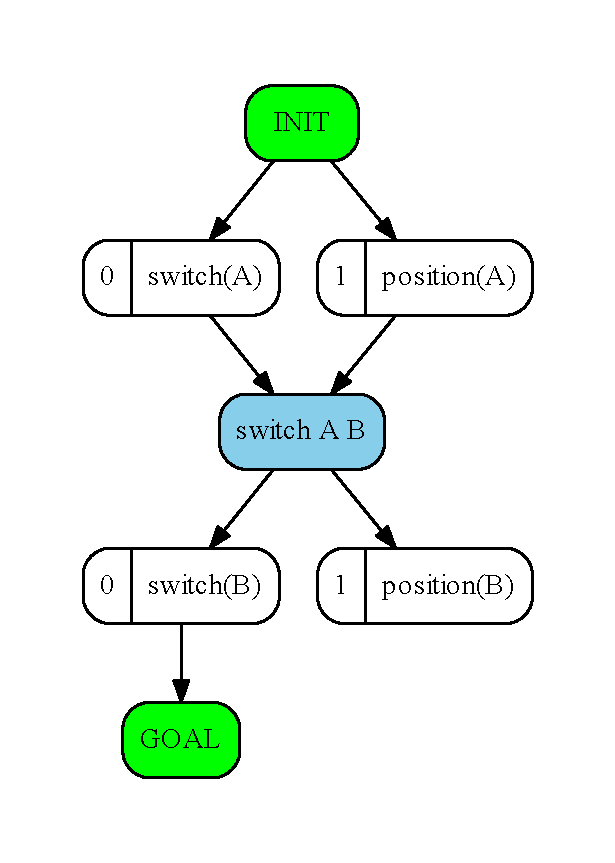
\includegraphics[scale=0.4]{oneEffectDelete/figures/simple_input}
			\caption{before reduction}
		\end{subfigure}	
		\begin{subfigure}[b]{0.4\textwidth}
			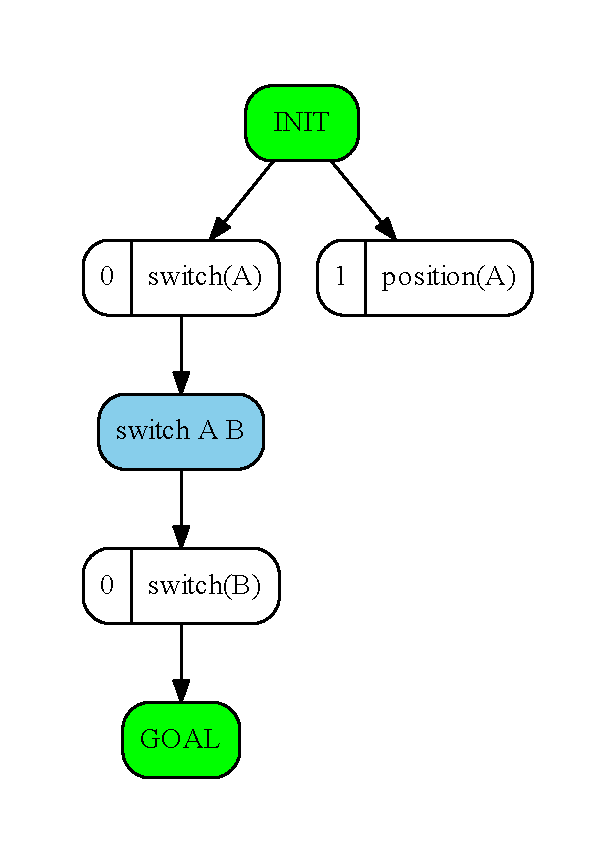
\includegraphics[scale=0.4]{oneEffectDelete/figures/simple_output}
		\caption{after reduction}
		\end{subfigure}
		\caption{Effect $<\emph{position(A)},\emph{position(B)}>$ can be removed from action \emph{switch A B} because effect $<\emph{switch(A)},\emph{switchtch(B)}>$ ensures that the action can be used at most once.}
	\end{figure}               
	
	
	
	\section{Reduce operation}
	Let's have SAS in form $<\vars, \init, \goal, \actions, \mutexes{}>$. There must be following values and actions in order to execute the action:
	
	\begin{enumerate}
		\item any value of variable $\var{u_i}$ is not in goal
		\item $u_i \in \init$
		\item $|\wan{u_i}| = 1$
		\item $|\pro{u_i}| = 0$
		\item $a \in \con{u_i}$
		\item $<u_i,u_j> \in \eff{a}$
		\item $|\con{u_j}| = 0$
		\item $<w_i,w_j> \ in \eff{a}, \var{w_i} \neq \var{v_i}$; action $a$ has another effect than $<u_i,u_j>$
		\item $|\con{w_j}| > 0$
		\item $|\pro{w_i}| = 0$
		\item $w_i \in \init$
	\end{enumerate}
	
	Action $a$ can be used only once, due to $<u_i, u_j>$. If there is another effect ($<w_i,w_j>$) that can be used only once, and its output ($w_j$) is used than the first effect can be omitted, because $u_j$ is not used in any other action. Also, there does not have to be any other action consuming $u_i$ or having it in prevail preconditon because of delete relaxation.
	
	
	The operation does following things:
	
	\begin{enumerate}
		\item $u_j$ is removed from $\dom{\var{u_j}}$
		\item $a_n \leftarrow <\pre{a}, \eff{a} \setminus \{<u_i,u_j>\}>$
		\item $\actions{}' \leftarrow (\actions \setminus \{a\}) \cup \{a_n\}$
	\end{enumerate}
	
	Output of the reduction is SAS $<\vars{}', \init{}, \goal{}, \actions{}', \mutexes{}>$.
	
	
	\section{Possible outgoing states of SAS}
	\begin{enumerate}
		\item states of SAS where -hc, -sd, -mo, -dv can be executed
	\end{enumerate}
	
	\section{States before application of this operation}
	\begin{itemize}
		\item original SAS
		\item after -ou, -mo, -dv, maybe others (-de)
		\item It seems that this operation is no longer needed when using -sf and -ai reductions, is it?
	\end{itemize}
	
	
	\section{Reverse operation}
	$a_n$ is removed from actions and $a$ is added back to the action set. Also, all occurrences of $a_n$ in plan are replaced by $a$.
		
	\section{Implementation notes}
	Simple implementation so far. There could be extension where $\var{u_i}$ is removed completely from the SAS (also actions that using $\var{u_i}$). It would be also faster.
	
	
	
	
	
	